
\documentclass[conference]{IEEEtran}
\IEEEoverridecommandlockouts
\usepackage{cite}
\usepackage{amsmath,amssymb,amsfonts}
\usepackage{algorithmic}
\usepackage{graphicx}
\usepackage{textcomp}
\usepackage{xcolor}
\usepackage{url}
\usepackage[hidelinks]{hyperref}

\begin{document}

\title{A Resource-Efficient Hardware Accelerator for Lossless Image
Compression Based on the Walsh--Hadamard Transform}

\author{
\IEEEauthorblockN{1\textsuperscript{st} Marco Zolla Salazar}
\IEEEauthorblockA{\textit{Maestría en Ingeniería Electrónica} \\
\textit{Instituto Tecnológico de Costa Rica}\\
Costa Rica \\ mzolla@estudiantec.cr}
\and
\IEEEauthorblockN{2\textsuperscript{nd} Luis Diego Martinez Jimenez}
\IEEEauthorblockA{\textit{Maestría en Ingeniería Electrónica} \\
\textit{Instituto Tecnológico de Costa Rica}\\
Costa Rica \\ diego\_mj22@estudiantec.cr}
\and
\IEEEauthorblockN{3\textsuperscript{rd} Simón Fallas Villalobos}
\IEEEauthorblockA{\textit{Maestría en Ingeniería Electrónica} \\
\textit{Instituto Tecnológico de Costa Rica}\\
Costa Rica \\ simonfallasv@estudiantec.cr}
\and[\hfill\mbox{}\\\mbox{}\hfill]
\IEEEauthorblockN{4\textsuperscript{th} Marcelo Mata Solano}
\IEEEauthorblockA{\textit{Maestría en Ingeniería Electrónica} \\
\textit{Instituto Tecnológico de Costa Rica}\\
Costa Rica \\ m.mata.3@estudiantec.cr}
\and
\IEEEauthorblockN{5\textsuperscript{th} Brandon Fabricio Rivera Hidalgo}
\IEEEauthorblockA{\textit{Maestría en Ingeniería Electrónica} \\
\textit{Instituto Tecnológico de Costa Rica}\\
Costa Rica \\ b.rivera.2@estudiantec.cr}
}

\maketitle

\begin{abstract}
This work presents forward and inverse hardware kernels for an integer and
reversible Walsh--Hadamard Transform used as a decorrelation stage in lossless
image compression. The lifting architecture relies on additions, subtractions,
and arithmetic shifts, which avoids multipliers while preserving exact
reconstruction. The synthesizable C++ functions matched a bit-accurate reference
model in 100,001 cases per direction, and the combined forward--inverse path
reconstructed 400,001 input blocks without error. C/RTL cosimulation passed for
the integrated and isolated kernels. In a controlled post-route comparison on an
AMD Kria KV260, the multiplier-free forward datapath used 501 LUTs, 424
flip-flops, no DSP blocks, and 1.5 BRAM tiles; the multiplier-based design used
500 LUTs, 377 flip-flops, 11 DSP blocks, and the same BRAM allocation. The
fastest tested constraints that closed timing were 250~MHz and 285.71~MHz,
respectively. Entropy experiments reduced the per-band entropy of spatially
correlated natural-like data by approximately 20\%. These results show that the
proposed transform removes DSP use with almost unchanged LUT cost, while trading
some register count and operating frequency.
\end{abstract}

\begin{IEEEkeywords}
Discrete transforms, Image coding, Data compression, Field programmable gate
arrays, Hardware acceleration, High level synthesis
\end{IEEEkeywords}

\section{Introduction}

Modern high-frame-rate camera systems, such as those deployed in intelligent vehicles and satellite imaging, generate massive volumes of data that must be processed and stored with minimal latency. In many of these edge-computing scenarios, lossless compression is essential because the uncertainty introduced by quantization noise in lossy systems is often inadmissible for maintaining system robustness or meeting legal requirements \cite{alonso2021}. Implementing these codecs in real-time at the edge is a critical challenge, as embedded video processors must handle high-speed transform computations while operating under strict limitations regarding hardware area, power consumption, and thermal dissipation \cite{amira2007}.

Transform methods are a fundamental component of image compression because they decorrelate spatial data before encoding, concentrating information into a smaller number of coefficients. Among these, the Walsh-Hadamard Transform (WHT) is particularly attractive for hardware implementations due to its significant computational advantages over sinusoidal transforms like the DFT or DCT. Because the WHT kernel matrix consists entirely of integer values of +1 and -1, the transform can be implemented very efficiently using only additions and subtractions, thereby eliminating the need for costly and time-consuming multipliers \cite{manjarres2021,hafizullah2018}.

Despite its advantages, state-of-the-art literature reveals limitations in existing solutions, which are frequently optimized for lossy applications or general neural network acceleration rather than resource-efficient lossless compression. For example, some high-throughput WHT-based architectures are designed for signal processing but rely on 32-bit floating-point arithmetic, which is not ideal for exact, low-resource lossless operation \cite{manjarres2021}. Conversely, other lossless approaches, such as those based on the JPEG-LS standard, provide competitive compression but often do not leverage the unique hardware-friendly properties of the WHT \cite{alonso2021}.

In this paper, we propose a resource-efficient integer/reversible WHT accelerator specifically designed for low-latency lossless compression. Our main contributions are:
\begin{itemize}
    \item An optimized integer/reversible WHT architecture that ensures mathematically exact data reconstruction for lossless applications.
    \item The development of a flexible design modeled at a high level using SystemC and HLS, allowing rapid design-space exploration and the generation of parallel-pipeline layouts.
    \item A reproducible FPGA evaluation that includes C/RTL cosimulation, post-route resource reports, and a controlled timing comparison against a multiplier-based implementation.
\end{itemize}

The remainder of this paper is organized as follows. Section II presents the background and related work. Section III describes the proposed architecture and its high-level implementation. Section IV reports the functional verification, entropy analysis, and hardware implementation results. Section V summarizes the conclusions, limitations, and future work.

\section{Background and Related Work}

The Walsh--Hadamard transform (WHT) decomposes a signal into Walsh basis functions
whose values are restricted to $\pm 1$. For a signal of $2^n$ samples the transform is
a multiplication by the $2^n \times 2^n$ Hadamard matrix, and since its entries are
$\pm 1$ it can be evaluated with additions and subtractions alone. The fast WHT (FWHT)
lowers the arithmetic cost from $O(N^2)$ to $O(N\log_2 N)$ through Cooley--Tukey-style
factorizations \cite{manjarres2021}, and its parallel-pipeline hardware implementations
follow processor structures first developed for the fast Fourier transform
\cite{wold1984}.

A conventional integer implementation of the WHT does not necessarily guarantee
lossless reconstruction because its inverse requires normalization by the transform
size $N$. This division may not be represented exactly using integer arithmetic,
causing information loss during a forward--inverse transform cycle. Integer, reversible formulations remove this limitation. The unified lossless
WHT (ULWHT) recovers the original data exactly while lowering the per-coefficient
entropy of natural images \cite{jung1997}, and a lossless two-dimensional WHT has also
been derived \cite{komatsu2001}. For hardware there is a caveat: the one-dimensional
lossless WHT still contains multiplications, and making it fully multiplier-free needs a
more elaborate construction \cite{komatsu2001}.

Two closely related solutions provide reproducible results with public code, and between
them they cover both sides of the problem. One is an FPGA WHT accelerator: a
configurable parallel-pipeline FWHT produced by high-level synthesis, with its HLS
source openly released \cite{manjarres2021}. The other is a parallel lossless compressor
for raw Bayer images on an FPGA-based high-speed camera that sustains $40.1$\,Gbit/s at
$320$\,MHz on a Zynq UltraScale+ device, using adaptive Golomb--Rice coding and a public
reference implementation \cite{regorsek2024}. One supplies the transform, the other a
low-latency lossless pipeline; bringing the two together is the open problem.

Five further works address parts of the problem. In hardware, a multiplier-free WHT
running at $162$\,MHz takes the place of the Photo Core Transform in JPEG~XR
\cite{hafizullah2018}, an FPGA JPEG\,2000 accelerator performs on-board lossless
compression \cite{ghodhbani2024}, and an ANS-based coder reduces the complexity of
JPEG-LS \cite{alonso2021}. The integer lossless WHT formulations achieve bit-exact
compression but stop at the algorithmic level, with no hardware realization
\cite{jung1997,komatsu2001}. Earlier WHT processors based on distributed arithmetic
\cite{amira2007}, the sequency-ordered complex Hadamard transform \cite{bi2008}, and a
radix-2 Walsh--Hadamard--Fourier pipeline \cite{liu2015} were built for high throughput
and small area, drawing on the low complexity of the $\pm 1$ kernel \cite{nayak2022}.

The WHT also appears outside compression, in image watermarking \cite{ho2003}, ultrasonic
coded excitation \cite{weng2024}, and the simulation of quantum algorithms
\cite{kobori2020}. To the best of the authors' knowledge, no recent FPGA accelerator combines
a reversible lossless WHT, a multiplier-free implementation, and publicly
reproducible results for high-frame-rate image processing.
The reproducible accelerators cover either the transform \cite{manjarres2021} or the
lossless coding \cite{regorsek2024}, and the lossless integer WHT has stayed at the
algorithmic level \cite{jung1997,komatsu2001}. Closing this gap is the aim of the present
work.






\section{Proposed Solution}
% blanca), cómo resuelve cada desafío, herramienta de modelado de III nivel.
\subsection{Study of Other Solutions in the State of the Art}

An analysis of recent literature over the past ten years reveals that implementations oriented 
toward image compression bifurcate into approaches that partially cover the problem but lack 
an efficient architectural integration specifically oriented toward a multiplier-free design 
for lossless video streams.

\subsubsection{Hardware Accelerators for Transforms (Lossy Approach)}
Hardware accelerators for transforms oriented toward lossy approaches have demonstrated 
remarkable efficiency in the real-time domain. These architectures achieve high data processing 
throughput by utilizing parallel and pipelined logic structures (\textit{parallel-pipeline}) \cite{manjarres2021},
also proving the physical feasibility of operating at high clock frequencies, such as $162\text{ MHz}$,
completely omitting advanced DSP logic blocks \cite{hafizullah2018}. Despite these strengths, 
these solutions present severe limitations when considered for lossless environments, as they
are optimized for generic processing or traditional lossy schemes relying on 32-bit 
floating-point arithmetic \cite{manjarres2021}. Furthermore, using the conventional inverse 
transform introduces division operations for normalization that integer-based systems cannot 
represent exactly, injecting quantization noise that destroys the possibility of exact data 
reconstruction \cite{jung1997}. Consequently, while these designs represent a valuable metric
baseline for evaluating hardware cost in terms of area and speed, they are not
directly suitable for strictly lossless compression applications.

\subsubsection{Lossless Hardware Compressors (Complete Pipelines)}
On the other hand, developments focused on complete lossless compression pipelines offer robust, 
low-latency alternatives essential for edge computing. Solutions such as parallel compressors 
for raw Bayer images implemented on FPGAs \cite{regorsek2024} and structural optimizations applied to the JPEG-LS standard under advanced coding architectures \cite{alonso2021} can sustain
massive data transfer rates in real-time. However, the main deficiency of this approach is that 
optimization efforts are directly concentrated on the entropy coding and packaging stages, 
omitting or completely replacing the spatial decorrelation phase based on discrete transforms 
such as the WHT \cite{alonso2021}. This omission makes them highly viable for general-purpose compression at the
edge, but not directly applicable when the architectural design goal is to
maximize datapath efficiency by exploiting a multiplier-free transformation core composed exclusively of $+1$ and $-1$ coefficients
\cite{hafizullah2018}.

\subsubsection{Reversible WHT Algorithmic Formulations}
Finally, proposals focused on the theoretical formulations of the reversible transform resolve the 
mathematical limitations of information loss in the inverse process. Mathematical models such as 
the unified lossless Walsh-Hadamard transform (ULWHT) and its two-dimensional derivations formally 
demonstrate that it is viable to recover data exactly bit-by-bit, significantly reducing the entropy 
per coefficient without resorting to complex multiplication operations \cite{jung1997, komatsu2001}. 
The major weakness of this approach lies in its purely abstract nature, given that these formulations 
have remained strictly in the algorithmic domain and lack a tangible realization or microarchitectural 
mapping in hardware for embedded systems \cite{jung1997}. Thus, although these formulations are suitable as numerical reference models,
they require hardware-oriented architectural redesign before direct FPGA implementation.

\subsection{Observed Challenges}

Based on the critical study of the state of the art, the fundamental architectural challenges that justify the contribution of this research are identified and outlined. The first challenge consists of properly delimiting the functional scope of the accelerator. Since the WHT transform acts solely as a spatial decorrelator and not as an autonomous codec, it is imperative to narrow the architecture to a dedicated transform core accelerator, structured in such a way that it can be seamlessly integrated into a larger lossless pipeline without diverting logic efforts toward complex entropy coding. The second technical challenge lies in performing a direct mapping from the abstract algorithmic domain to a real physical architecture with zero use of DSP blocks. Although the literature describes theoretical reversible and multiplier-free versions \cite{komatsu2001}, their implementation through high-level synthesis (SystemC/HLS) requires optimizing subexpression reuse and designing aggressive pipelining to mitigate FPGA resource consumption.

As a third challenge, there is a need to strongly justify the choice of the WHT over competing integer transforms such as the DCT or wavelets. Because the WHT exhibits inferior performance in lossy compression quality \cite{regorsek2024}, the proposed architecture must be empirically evaluated in terms of logic area cost and maximum operating frequency in a lossless environment. The fourth challenge focuses on ensuring real-time operational performance for high-frame-rate video streams, which forces the design of a datapath with a highly optimized transaction-level data flow that minimizes stall cycles under the strict thermal and power constraints of embedded systems \cite{amira2007}. Finally, the fifth challenge corresponds to the verification of bit-exact
reproducibility. To ensure identical reconstruction of the original data, a
bit-accurate SystemC reference model was developed and used as the verification
oracle for deterministic and randomized comparisons against the HLS implementation.


\subsection{Scope and Design Philosophy}
Based on the analysis presented in Section II, this work addresses the limited availability of recent FPGA accelerators that combine a reversible WHT, multiplier-free arithmetic, and reproducible implementation results. Therefore, this work focuses on the development of an accelerator dedicated exclusively to the execution of the transform.
The proposed system performs an integer and reversible Walsh-Hadamard Transform on pixel blocks obtained from a high-speed video stream. The output consists of transform coefficients that can subsequently be processed by an entropy coding stage, such as Golomb-Rice or ANS coding.
This design boundary allows the evaluation of only the hardware associated with the transform itself, quantifying its efficiency in terms of resource utilization and performance without being influenced by the compression ratio of a complete codec.
\subsection{High-Level Architecture}

The proposed architecture consists of five main functional blocks, as illustrated in Fig.~\ref{fig:wht_architecture}.
\begin{figure}[htbp]
\centering
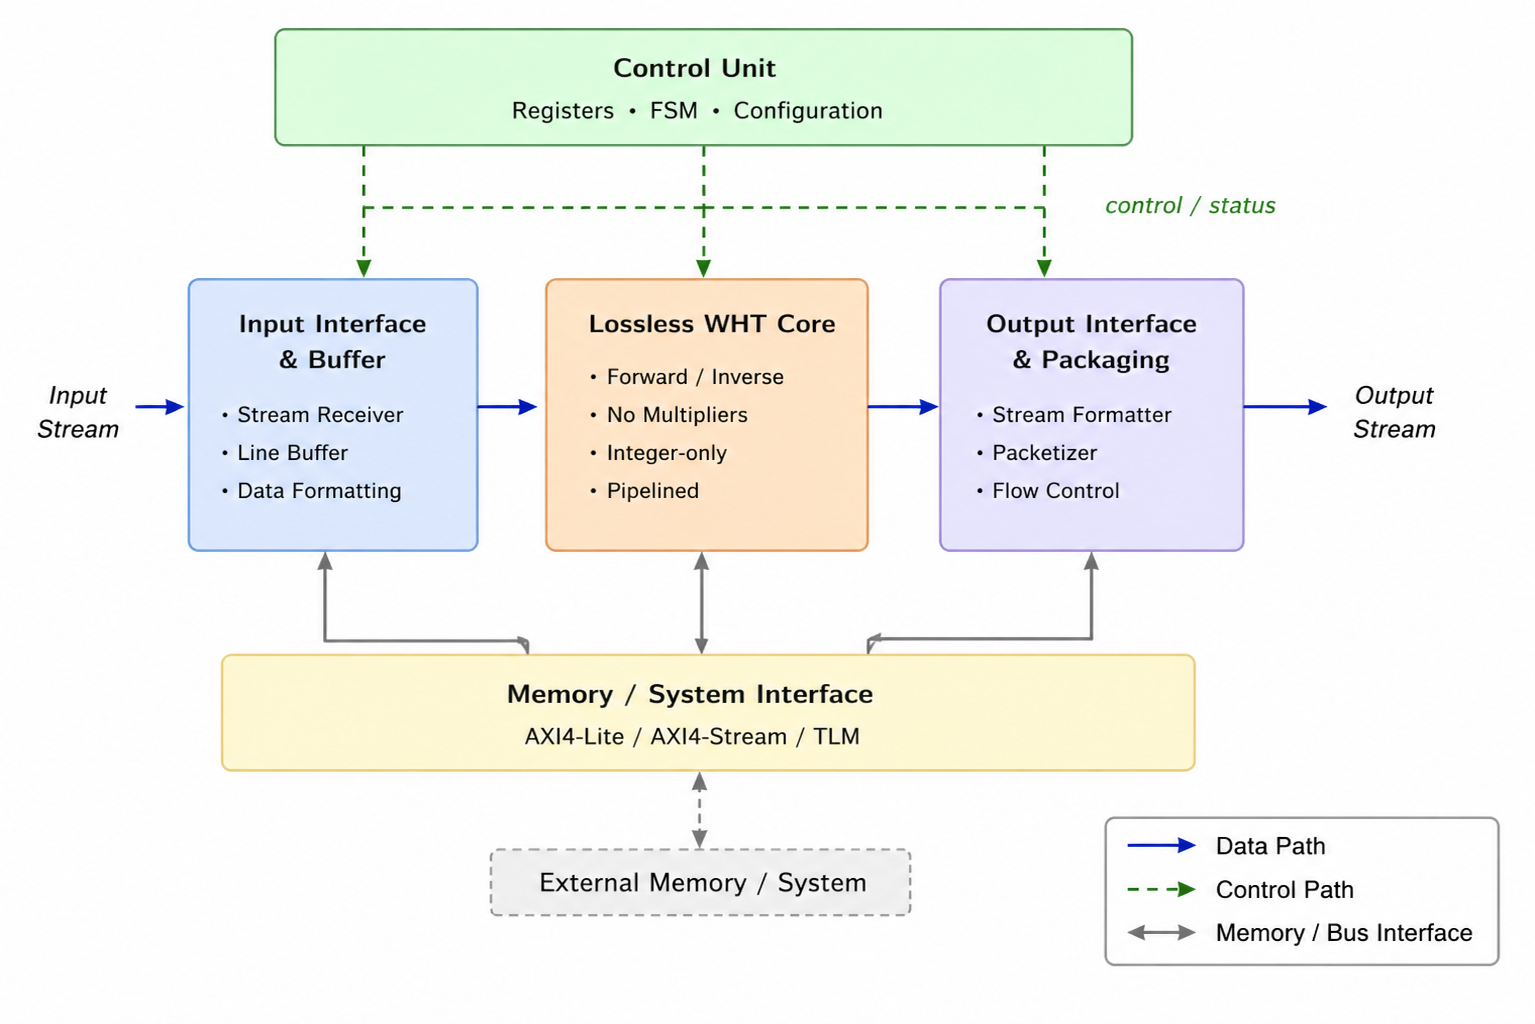
\includegraphics[width=0.42\textwidth]{wht_architecture.png}
\caption{High-level architecture of the proposed lossless WHT accelerator.}
\label{fig:wht_architecture}
\end{figure}

\subsubsection{Input Buffer and Interface (IF)}

This block receives pixels from the camera or memory subsystem and organizes them into transform blocks. The implemented architecture uses a block size of $N=8$, selected as a practical compromise between hardware complexity, latency, and verification effort.

\subsubsection{Lossless WHT Core}

The computational core of the accelerator was designed in Vitis HLS utilizing a fully parallel, multiplier-free architecture. To satisfy the requirements of a lossless environment (zero quantization noise) while keeping DSP utilization at zero, the standard fast Walsh-Hadamard butterfly was replaced by an integer lifting-based scheme (S-Transform) \cite{jung1997}. 

The fundamental spatial decorrelation step between two pixels $a$ and $b$ is implemented purely through high-frequency differences ($d = a - b$) and low-frequency shifted averages ($s = a - (d \gg 1)$). This specific subexpression routing is synthesized by the HLS compiler completely into LUTs and Flip-Flops, bypassing any DSP slice instantiation.

To expose parallelism, the $N=8$ transform is written as three fully unrolled combinational butterfly stages. The integrated top functions use \texttt{m\_axi} memory interfaces and request an initiation interval of one through \texttt{\#pragma HLS PIPELINE II=1}. HLS achieved a latency of 143 cycles and $II=1$ for both AXI tops. The datapath uses \texttt{ap\_int<16>} to limit the arithmetic width while preserving the verified 8-bit input range.

Forward and inverse operations are provided as separate synthesizable top functions. Additional \texttt{ap\_memory} versions isolate the butterfly datapath from the AXI wrapper. These isolated variants allow a controlled comparison with the multiplier-based design under matching interfaces and constraints. The complete HLS source and reports are available in the public repository \cite{repo_grupo5}.

\subsubsection{Control Unit}

The control unit manages the overall operation of the accelerator. Although it does not directly perform the WHT computation, it coordinates when pixel blocks enter the system, when temporary data are stored in registers, and when results are forwarded to the next pipeline stage. Furthermore, it synchronizes processing to prevent data conflicts and enables architectural parallelism through control signals such as enable, valid, and ready.

\subsubsection{Output Interface and Packaging}

This module collects the transformed coefficients and packages them for transmission or subsequent entropy coding. Like the input buffer, it is part of the system-level integration.

\subsubsection{Memory Interface (AXI4/AXI4-Lite)}

This module manages data transfers between the accelerator and the external memory subsystem. The use of AXI4 and AXI4-Lite interfaces facilitates integration into FPGA-SoC platforms such as the Kria KV260 and Alveo U55C, allowing the accelerator to be incorporated into larger embedded processing systems.

The current implementation and evaluation focus on the WHT computational core. The control unit, input buffering, output packaging, and external-memory interfaces remain part of the proposed system-level integration and were not independently evaluated in the reported experiments.

\subsection{Challenge--Solution Mapping}

The proposed architecture aims to address the main challenges identified during the literature review. Table~\ref{tab:challenge_solution} summarizes how each challenge is considered within the proposed solution.

\begin{table}[htbp]
\caption{Challenge--Solution Mapping}
\label{tab:challenge_solution}
\centering
\begin{tabular}{|p{2.1cm}|p{5.2cm}|}
\hline
\textbf{Challenge} & \textbf{Proposed Solution} \\
\hline

D1 -- Codec Scope &
This work focuses only on the WHT stage. Entropy coding (e.g., Golomb-Rice, ANS) is considered a later processing stage, allowing the transform hardware to be evaluated independently.
\\ \hline

D2 -- DSP-Free FPGA Implementation &
The WHT core uses only additions, subtractions, and arithmetic right shifts based on the lifting construction from \cite{jung1997}, minimizing DSP usage and mapping entirely to LUTs and Flip-Flops.
\\ \hline

D3 -- Hardware relevance &
The multiplier-free datapath is compared with an equivalent multiplier-based implementation using the same target, interfaces, and implementation flow.
\\ \hline

D4 -- Real-Time Throughput &
The AXI forward and inverse tops achieve $II=1$, while the isolated datapaths and multiplier baseline achieve $II=9$. A timing sweep reports the fastest tested clock constraint that closes routing.
\\ \hline

D5 -- Bit-Exact Lossless Reconstruction &
The reversible lifting formulation is checked against a bit-accurate C++ reference model and by an end-to-end forward--inverse test. C/RTL cosimulation also passes for the implemented variants.
\\ \hline

\end{tabular}
\end{table}

Overall, the proposed architecture provides a feasible FPGA implementation of a lossless Walsh-Hadamard Transform while addressing the main limitations identified in previous studies.


\section{Results and Analysis}

This section presents the experimental methodology used to evaluate the proposed
accelerator and to contrast it against the state of the art, covering the modeling
and synthesis toolchain, the experiments and baselines, and the metrics collected
for the comparison. In addition to entropy and bit-exactness checks, we report 
post-route FPGA metrics.

\subsection{Experimental Setup and Toolchain}
The verification oracle is a bit-accurate C++ golden model, with a SystemC wrapper used for the forward-path demonstration. The forward and inverse synthesizable functions were compared against the golden implementation at the C/C++ source level before RTL synthesis. Portable regression tests use the repository's \texttt{ap\_int} compatibility layer when the Vitis headers are unavailable; consequently, this evidence does not replace C/RTL cosimulation.

The HLS and Vivado scripts target the AMD Kria~KV260 (Zynq UltraScale+ MPSoC, part \texttt{xck26-sfvc784-2LV-c}). HLS uses a 4~ns target period. Vivado first implements each variant with a 10~ns constraint; the controlled forward comparison also routes the same RTL at 6.0, 5.0, 4.5, 4.0, 3.5, and 3.0~ns. The fastest tested period with non-negative WNS is reported as a demonstrated bound rather than an exact $f_{\max}$. No measurements were performed on a physical board.

\subsection{Experiments and Baselines}
All software experiments are reproducible from the public repository \cite{repo_grupo5}: 
the reference model, the test benches, and the datasets are generated 
deterministically from a fixed seed. The evaluation uses five 8-bit grayscale 
$256\times256$ images spanning the range of spatial correlation: a constant field, 
a linear ramp, a piecewise-constant image with sharp edges, a $1/f$ surface with 
spatial correlation similar to natural images, and white noise as a control. The 
transform is applied over one-dimensional $N=8$ strips, matching the hardware; 
a separable two-dimensional variant (row then column) is also evaluated as a 
software-only extension.

The repository includes two baselines. A conventional C++ FWHT serves as a functional reference. A reversible multiplier-based lifting design provides the hardware comparison. The proposed and multiplier-based forward datapaths use matching \texttt{ap\_memory} interfaces, the same Kria KV260 part, the same HLS target, and the same Vivado flow. Their C/RTL cosimulations and post-route implementations completed successfully.

\subsection{Evaluation Metrics}
Two metric axes were collected (Table~\ref{tab:expplan}). Hardware efficiency was 
measured by look-up table (LUT), flip-flop (FF), and DSP-block utilization, the 
maximum operating frequency ($f_{\max}$), processing latency, and throughput in 
operations per second. 
Compression behavior was assessed by bit-exact lossless verification against the 
golden model and by the per-coefficient entropy reduction in bits per symbol.

\begin{table}[htbp]
\caption{Evaluation Metrics}
\label{tab:expplan}
\centering
\begin{tabular}{@{}ll@{}}
\hline
\textbf{Axis} & \textbf{Metrics} \\
\hline
Hardware cost & LUT, FF, DSP, $f_{\max}$, latency, throughput (OP/s) \\
Compression   & bit-exact verification, entropy reduction (bits/pixel) \\
\hline
\end{tabular}
\end{table}

\subsection{Functional Verification}
Verification was performed at the C/C++ source level before RTL synthesis. The
forward kernel matched the golden forward transform in one fixed case and
100,000 random 8-bit blocks (100,001/100,001). The inverse kernel independently
matched the golden inverse transform in 100,001 full-range signed 16-bit cases.
A separate end-to-end test directly linked the two synthesizable functions and
verified
\(\texttt{inverse\_core}(\texttt{forward\_core}(x))=x\) in 400,001 cases.
Therefore, exact reconstruction is supported by the actual forward and inverse
source functions, rather than only by a round trip internal to the golden model.
The portable regression uses the repository's \texttt{ap\_int} compatibility
layer when Vitis headers are unavailable. This source-level evidence is
complemented by XSim C/RTL cosimulation, which passed for the AXI forward and
inverse kernels, the isolated forward and inverse datapaths, and the
multiplier-based forward design.

\subsection{Entropy Reduction}
Since the accelerator implements the transform stage only, its benefit is
measured as the reduction in zeroth-order entropy (bits per symbol) between the
pixels and the transform coefficients. Entropy is the lower bound on the rate of
any zeroth-order lossless coder, so a lower value indicates more compressible
data. The length-8 transform maps each block to one DC (mean) coefficient and
seven detail coefficients of increasing sequency, which we treat as eight
frequency bands. We report a pooled estimate (all coefficients in one histogram) and a
per-band estimate (one entropy per frequency position, averaged), the latter
being closer to the cost of a coder that models each band separately.
Table~\ref{tab:entropy} lists the results.

\begin{table}[htbp]
\caption{Zeroth-order entropy (bits/symbol): pixels vs.\ WHT coefficients.}
\label{tab:entropy}
\centering
\begin{tabular}{|l|c|cc|cc|}
\hline
 & & \multicolumn{2}{c|}{1D ($N{=}8$, HW)} & \multicolumn{2}{c|}{2D separable} \\
Dataset & $H_{\mathrm{pix}}$ & pool & band & pool & band \\
\hline
Flat    & 0.00 & 0.54 & 0.00 & 0.12 & 0.00 \\
Ramp    & 8.00 & 2.63 & 0.63 & 0.54 & 0.08 \\
Edges   & 2.00 & 0.79 & 0.25 & 0.15 & 0.03 \\
Natural & 7.30 & 6.55 & 5.81 & 5.86 & 5.31 \\
Noise   & 8.00 & 8.75 & 8.20 & 8.77 & 7.84 \\
\hline
\end{tabular}
\end{table}

The reduction tracks the spatial correlation of the input. Smooth images (ramp,
edges) concentrate almost all information in the DC band and drive the detail
bands to zero entropy, giving per-band reductions of $87$--$92\%$. For the
natural-like image the per-band reduction is $20\%$ in one dimension and $27\%$
for the separable two-dimensional transform. White noise, having no spatial
correlation, is not improved by the transform and serves as a control; its
coefficient entropy even exceeds the 8 bits of the input because the
coefficients span a wider dynamic range than the pixels, which is also why the
datapath is 16 bits wide. The gap
between the one- and two-dimensional results motivates a two-dimensional core as
future work.

A software-only one-dimensional block-size sweep was also performed for
\(N\in\{8,16,32\}\). For the natural-like dataset, the per-band entropy changed
from 5.808 to 5.721 and 5.674 bits/symbol, respectively. No overflow was found in
any of the 15 dataset/size combinations. This sweep demonstrates the software
behavior and the adequacy of the 16-bit range, but only the \(N=8\) architecture
has been implemented in hardware.

\begin{figure}[htbp]
\centering
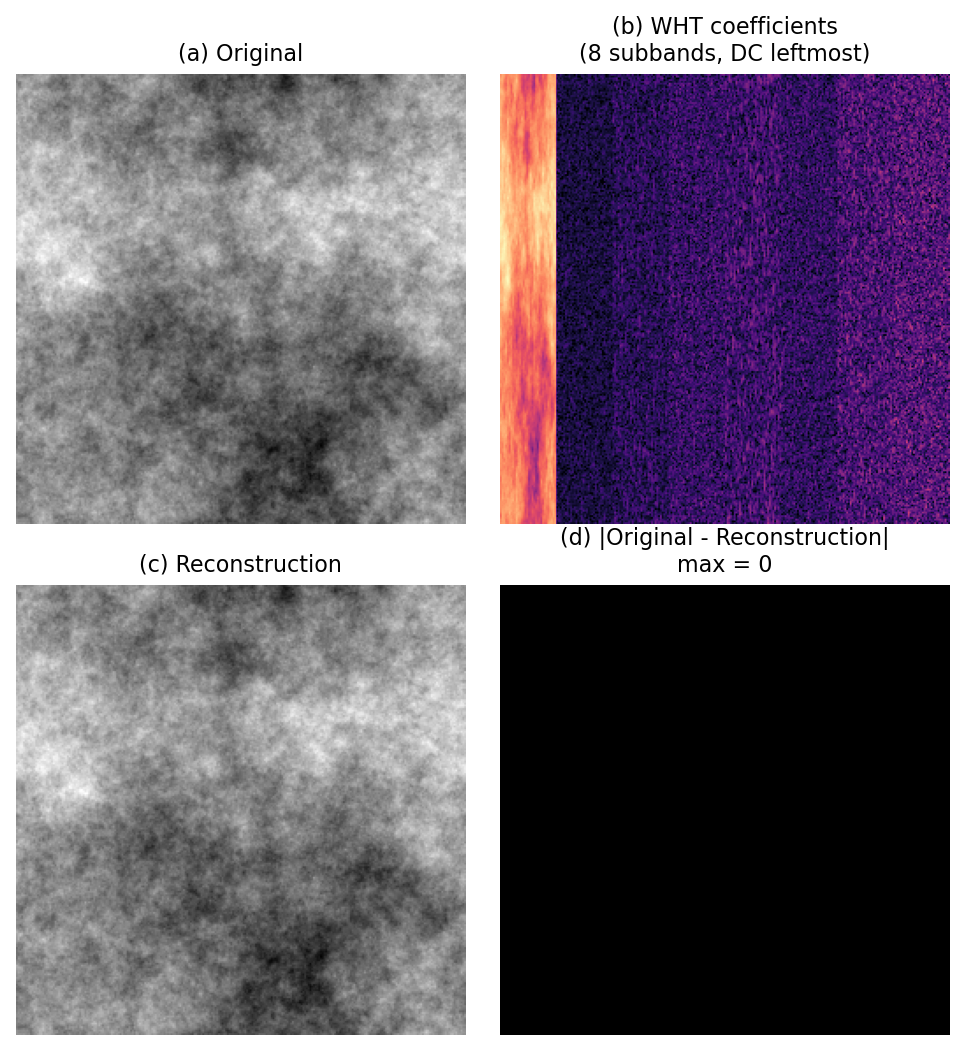
\includegraphics[width=\columnwidth]{wht_reconstruction.png}
\caption{Software visualization for the natural-like dataset: original image,
1D WHT coefficients grouped by subband, exact reconstruction, and absolute
difference. The maximum reconstruction error is zero.}
\label{fig:reconstruction}
\end{figure}

\subsection{Hardware Implementation Results}
All five evaluated variants completed HLS synthesis, XSim C/RTL cosimulation,
and out-of-context Vivado implementation. Table~\ref{tab:controlled} compares
the isolated forward datapath with the multiplier-based forward design. Both
use the same target part, memory-style interfaces, HLS clock target, and Vivado
flow.

\begin{table}[htbp]
\caption{Controlled forward comparison on the Kria KV260.}
\label{tab:controlled}
\centering
\begin{tabular}{@{}lrr@{}}
\hline
\textbf{Metric} & \textbf{Multiplier-free} & \textbf{Multiplier-based} \\
\hline
HLS latency (cycles) & 17 & 17 \\
HLS initiation interval & 9 & 9 \\
HLS LUT & 880 & 926 \\
HLS FF & 562 & 823 \\
HLS DSP & 0 & 12 \\
Post-route LUT & 501 & 500 \\
Post-route FF & 424 & 377 \\
Post-route DSP & 0 & 11 \\
Post-route BRAM (tiles) & 1.5 & 1.5 \\
Demonstrated frequency (MHz) & 250.00 & 285.71 \\
\hline
\end{tabular}
\end{table}

The multiplier-free core removes all 11 routed DSP blocks while keeping LUT
utilization essentially unchanged. It uses 47 additional flip-flops and reaches
a lower demonstrated frequency. Relative to the multiplier-free result, the
multiplier-based design closes at a 14.3\% higher tested frequency. These values
are the fastest constraints in the evaluated sweep that completed routing with
non-negative WNS: 4.0~ns with 0.157~ns WNS for the proposed datapath and 3.5~ns
with 0.089~ns WNS for the baseline.

The isolated inverse datapath also completed C/RTL cosimulation and routing. It
uses 565 LUTs, 409 flip-flops, no DSP blocks, and 1.5 BRAM tiles, with a
17-cycle latency and $II=9$ in HLS.

Table~\ref{tab:axi} reports the two AXI-integrated kernels. Their larger resource
counts are mainly associated with the memory and control interfaces, so they are
not used in the controlled datapath comparison.

\begin{table}[htbp]
\caption{AXI-integrated forward and inverse kernels.}
\label{tab:axi}
\centering
\begin{tabular}{@{}lrr@{}}
\hline
\textbf{Metric} & \textbf{Forward} & \textbf{Inverse} \\
\hline
HLS latency (cycles) & 143 & 143 \\
HLS initiation interval & 1 & 1 \\
HLS LUT & 1773 & 1773 \\
HLS FF & 1847 & 1907 \\
Post-route LUT & 2340 & 2366 \\
Post-route FF & 2716 & 2716 \\
Post-route DSP & 0 & 0 \\
Post-route BRAM (tiles) & 4 & 4 \\
WNS at 10~ns (ns) & 4.292 & 5.980 \\
\hline
\end{tabular}
\end{table}

Vivado also generated vectorless power estimates. Because no switching-activity
file or board measurement was used, those figures are treated as implementation
estimates and are not used to claim measured energy efficiency.

\section{Conclusions and Future Work}
This work implements separate forward and inverse length-8 reversible WHT
kernels using a multiplier-free lifting construction. The source functions
matched the reference model in 100,001 cases per direction, completed 400,001
exact forward--inverse reconstructions, and passed C/RTL cosimulation. The
entropy experiment produced a 20\% per-band reduction for the natural-like
dataset, while the software sweep completed $N\in\{8,16,32\}$ without overflow.

Under matched implementation conditions, the multiplier-free forward datapath
eliminated 11 routed DSP blocks while using nearly the same LUT count as the
multiplier-based design. Its cost was 47 additional flip-flops and a maximum
demonstrated frequency of 250~MHz instead of 285.71~MHz. The isolated inverse
and both AXI-integrated kernels also routed with zero DSP usage, supporting the
implementation of the reversible path in hardware.

The current system remains a transform accelerator rather than a complete image
codec. Buffering, entropy coding, camera integration, and packetization are
outside the evaluated core. The power reports are vectorless estimates, and no
physical-board measurements were performed. Future work includes a separable
2D hardware implementation, synthesized support for larger block sizes, tests
with real camera frames, integration with an entropy coder, and measurements on
the target board.

\section*{Declaration on the Use of Generative AI}
Generative tools were used for language review, reference formatting, and
consistency checks. The authors reviewed the cited sources, executed the tests
and hardware flows, verified the numerical results, and remain responsible for
the technical content and conclusions.

\begin{thebibliography}{00}
\bibitem{manjarres2021} A. Manjarres Garcia, C. Osorio Quero, J. Rangel-Magdaleno, J. Martinez-Carranza, and D. Durini Romero, ``Parallel-pipeline fast Walsh-Hadamard transform implementation using HLS,'' in \emph{Proc. Int. Conf. Field-Programmable Technology (ICFPT)}, 2021, doi: 10.1109/ICFPT52863.2021.9609874.
\bibitem{jung1997} H.-Y. Jung, R. Prost, and T.-Y. Choi, ``A unified mathematical form of the Walsh--Hadamard transform for lossless image data compression,'' \emph{Signal Process.}, vol. 63, pp. 35--43, 1997, doi: 10.1016/S0165-1684(97)00138-2.
\bibitem{komatsu2001} K. Komatsu and K. Sezaki, ``Lossless 2D discrete Walsh-Hadamard transform,'' in \emph{Proc. IEEE Int. Conf. Acoust., Speech, Signal Process. (ICASSP)}, 2001, doi: 10.1109/ICASSP.2001.941320.
\bibitem{hafizullah2018} S. Hafizullah, M. S. S. V. S. Manideep, V. Sharma, P. K. Nath, A. Naugarhiya, and S. Verma, ``An efficient hardware implementation of Walsh Hadamard transform for JPEG XR,'' in \emph{Proc. 15th IEEE India Council Int. Conf. (INDICON)}, 2018, doi: 10.1109/INDICON45594.2018.8987180.
\bibitem{regorsek2024} \v{Z}. Regor\v{s}ek, A. Gorki\v{c}, and A. Trost, ``Parallel lossless compression of raw Bayer images on FPGA-based high-speed camera,'' \emph{Sensors}, vol. 24, no. 20, art. 6632, 2024, doi: 10.3390/s24206632.
\bibitem{ghodhbani2024} R. Ghodhbani, T. Saidani, L. Horrigue, A. M. Algarni, and M. Alshammari, ``An FPGA accelerator for real-time hyperspectral image compression based on JPEG2000 standard,'' \emph{Eng. Technol. Appl. Sci. Res.}, vol. 14, no. 2, pp. 13118--13123, 2024, doi: 10.48084/etasr.6853.
\bibitem{alonso2021} T. Alonso, G. Sutter, and J. E. L\'opez de Vergara, ``LOCO-ANS: An optimization of JPEG-LS using an efficient and low-complexity coder based on ANS,'' \emph{IEEE Access}, vol. 9, pp. 106606--106626, 2021, doi: 10.1109/ACCESS.2021.3100747.
\bibitem{nayak2022} D. Nayak, K. Ray, T. Kar, and C. Kwan, ``Walsh--Hadamard kernel feature-based image compression using DCT with bi-level quantization,'' \emph{Computers}, vol. 11, no. 7, art. 110, 2022, doi: 10.3390/computers11070110.
\bibitem{weng2024} C. Weng, X. Gu, and H. Jin, ``Coded excitation for ultrasonic testing: A review,'' \emph{Sensors}, vol. 24, no. 7, art. 2167, 2024, doi: 10.3390/s24072167.
\bibitem{kobori2020} A. Kobori, R. Takahashi, and M. Nakanishi, ``A hardware architecture for the Walsh--Hadamard transform toward fast simulation of quantum algorithms,'' \emph{CCF Trans. High Perform. Comput.}, vol. 2, pp. 211--220, 2020, doi: 10.1007/s42514-020-00028-7.
\bibitem{amira2007} A. Amira and S. Chandrasekaran, ``Power modeling and efficient FPGA implementation of FHT for signal processing,'' \emph{IEEE Trans. Very Large Scale Integr. (VLSI) Syst.}, vol. 15, no. 3, pp. 286--295, 2007, doi: 10.1109/TVLSI.2007.893606.
\bibitem{bi2008} G. Bi, A. Aung, and B. P. Ng, ``Pipelined hardware structure for sequency-ordered complex Hadamard transform,'' \emph{IEEE Signal Process. Lett.}, vol. 15, pp. 401--404, 2008, doi: 10.1109/LSP.2008.922515.
\bibitem{liu2015} J. Liu, Q. Xing, X. Yin, X. Mao, and F. Yu, ``Pipelined architecture for a radix-2 fast Walsh--Hadamard--Fourier transform algorithm,'' \emph{IEEE Trans. Circuits Syst. II, Exp. Briefs}, vol. 62, no. 11, pp. 1083--1087, 2015, doi: 10.1109/TCSII.2015.2456371.
\bibitem{wold1984} E. Wold and A. Despain, ``Pipeline and parallel-pipeline FFT processors for VLSI implementations,'' \emph{IEEE Trans. Comput.}, vol. C-33, no. 5, pp. 414--426, 1984, doi: 10.1109/TC.1984.1676458.
\bibitem{ho2003} A. T. Ho, J. Shen, A. K. Chow, and J. Woon, ``Robust digital image-in-image watermarking algorithm using the fast Hadamard transform,'' in \emph{Proc. Int. Symp. Circuits Syst. (ISCAS)}, 2003, doi: 10.1109/ISCAS.2003.1205147.
\bibitem{repo_grupo5} MP-6160 Grupo 5, ``WHT Lossless Accelerator Repository.'' [Online]. Available: \url{https://github.com/TorikTheGreat/MP6160_grupo_5/tree/wht_accelerator_project}
\end{thebibliography}

\end{document}
